\documentclass[runningheads]{llncs}
\usepackage{graphicx}
\usepackage[
    left=3cm,
    right=3cm,
    top=4cm,
    bottom=4cm
]{geometry}

\begin{document}

% Comparing the Effectiveness of Deep Learning Models
% on the Categorisation of Galaxy Morphology
\title{
    Comparing the Effectiveness of Deep Learning Models on the Categorisation of Galaxy Morphology
    \\ CMP3753M Project Proposal
}

\author{Luke Roberts}

\institute{University of Lincoln \\
\email{25722923@students.lincoln.ac.uk}}

\maketitle

\section{Introduction}
%   Overview
% - Introduce key concepts like deep learning and
%   image classification, and why they are relevent
%   to study -> What are their uses?
%
% - Introduce galaxy morphology and the importance of
%   further studying distant galaxies for bettering
%   human understanding of the cosmos -> Why is it important?
%
% - Link the two ideas and showcase previous research,
%   adding references when appropriate
%
%   Paragraph 1
% - What is deep learning and image classification
% - Image classification accurately (but not always perfectly)
%   catagorise images in a specific dataset
% - (we will be using a specific dataset of images)
% - Different image classification models work better with
%   different themed image sets
%
%   Paragraph 2
% - Astronomy and understanding the universe is important
%   for scientific research
% - Understanding galaxy forms is a small but important part
%   of astronomy
% - Because of the massive amount of data produced by
%   observatries e.g. the hubble space telescope, it takes
%   a long time for people to accurately catagorise the
%   growing dataset.
% - There exists databases of already catagorised
%   galaxies
% - We should therefore use this data to catagorise new
%   images of galaxy morphology
%
%   Conclusion
% - We should analise which Deep Learning Model is best for
%   catagorizing galaxies into different morphologies.

Introduction

Understanding the universe has been a pursuit of humanity for thousands of
years. Because of the increasing effectiveness of deep learning image
classification models, categorising distant objects in space has become much
easier. Therefore, this rapid development in deep learning will allow
astrophysicists to further their research into the early universe.

Due to advances in observational technology such as the Hubble Space Telescope
(HST) and more recently the James Webb Space Telescope (JWST) [], we can observe
galaxies billions of lightyears from earth. The time taken for the light of
distant galaxies to reach us means that our night sky is a window into the
past, which allows astrophysicists to understand the evolution of our universe
in more depth []. Photographs such as the Hubble Ultra-Deep field show us an
ancient universe full of developing galaxies [], and the amount of observed
galaxies in astronomy databases is only increasing.

By identifying how the structure of galaxies, or galaxy morphology, changes over
 time, we have a clearer picture of the changes of galactic structure over the
 last several billion years. However, it is extremely time-consuming for
 scientists to categorise galaxies in their research. A study in 2016 []
 calculated that there are ~2.0×10¹² galaxies in the observable universe. While
 it would be unfeasible to categorise them all, it would be much more efficient
 to automate the process. One powerful method for automation of images is to
 train and deploy a deep learning model.

Deep Learning has recently revolutionised both scientific research and modern
life in a profound way []. From the categorisation of X-ray images in the
medical field; machine translation of natural language such as Google Translate
and large large language models such as ChatGPT, deep learning has become the
best way to categorise, analyse and generate unstructured data []. To perform
many of these tasks, machine learning engineers create deep learning models
which utilise a dataset that learns patterns about that data.

Image classification is a form of deep learning that uses images as input data
and is used for a wide variety of applications in scientific research []. Like
all forms of deep learning, image processing models are trained so that they
more accurately categorise new input data []. At the start of training, the
model performs poorly when tested. However, through analysing how the output
fails, the model can tweak its own parameters in order to achieve greater
accuracy []. The choice of which machine learning model or architecture to use
and the specific hyperparameters are important for maximising the efficiency of
the model []. This can be due to the content and quality of the training data
being used.

Recent studies such as ‘Galaxy classification: deep learning on the OTELO and
COSMOS databases’ [] concluded that using a DNN “outperforms” other adopted
models for galaxy classification. However, to extend this research I will
evaluate which deep learning neural network is most effective at classifying
the morphology of distant galaxies by implementing deep learning architectures
and evaluating their computational efficiency and performance in categorisation.

\section{Aims and Objectives}

\subsection{Aim}
One of the most widely adopted deep learning image classification is the
convolutional neural network (CNN) [] which has been used in many studies to
categorise a wide range of image types. New deep learning image classification
architectures have been developed which have either greater accuracy or are
faster at categorising data. ConvXGB has been shown to improve on
CNNs [Tables 5a-c] for different datasets. The aim of this project is to
determine which deep learning model is more suitable to classify deep space
galaxy morphology from existing databases of galaxy images. This will be
training the models and calculating ML performance heuristics.

\subsection{Objectives}

\begin{enumerate}
    \item Gather a dataset of galaxy images, coupled with their morphological
    type. I will use an official astronomy database like the ESA astronomy
    archives [] using the python astroquery library []. The dataset of images
    needs to be analysed to see if formatting it is necessary.

    \item Implement a method of preprocessing images for training in python
    through an image procseeing library such as PIL [].

    \item Implement deep learning models (NN, CNN, ConvXGB) for predicting
    the categorisation of images of galaxies. The real type of morphology
    associated with that image will be used in backpropergation the of the model
    to train it. This will be done using the python libraries Sci-kit Learn [],
    TensorFlow [] and XGBoost []. GPU parallelisation will be needed to train
    the dataset much more quickly.

    \item Split the dataset into training and testing. Train the models with the
    training dataset gathered. Models will be tested using the testing dataset
    and ML performance heuristics will be calculated. The performance heuristics
    will determine which model is better at categorising galaxy morphology.
    Additionally at this stage some hyperparameter tuning will be performed to
    improve model performance.
\end{enumerate}

\section{Project Plan and Risk Analysis}

\subsection{Project Plan}

In the project I will concurrently work on both the practical implementations
and disertation writing. Each stage of the implementation will be done in the
order stated above in Objectives and an appropriate amount of time is given to
each task depending on the complexity.

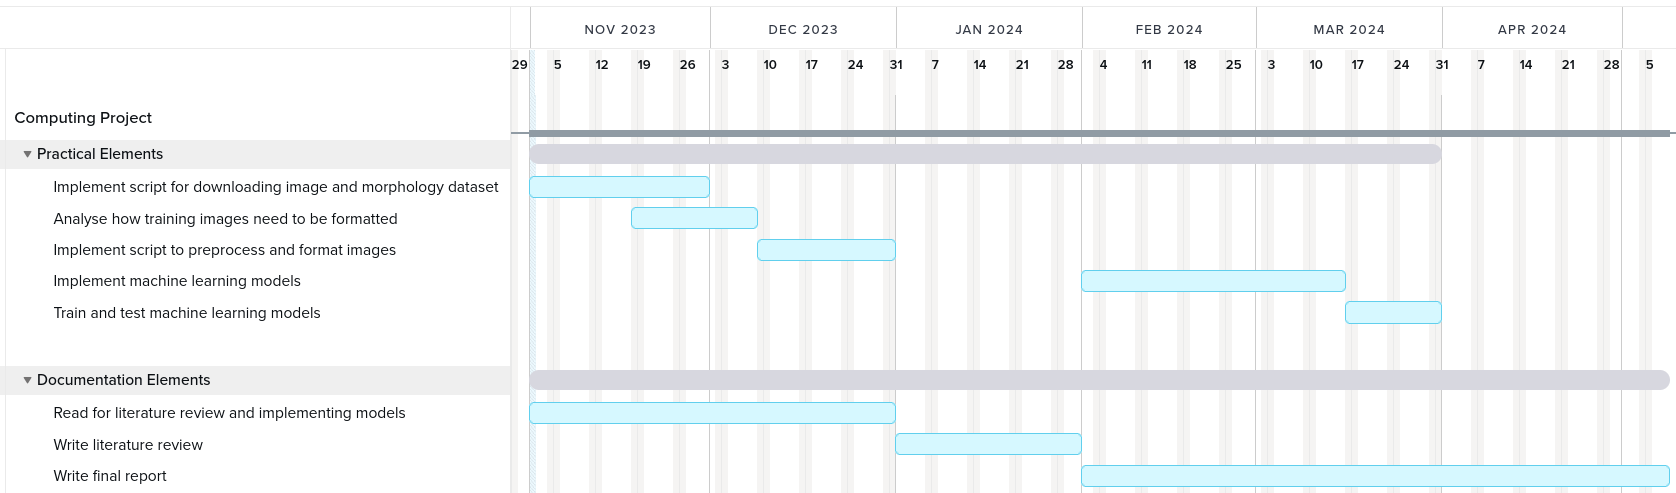
\includegraphics[width=\textwidth]{GantChart.png}
Gant Chart of project

\subsection{Risk Analysis}

\begin{table}
    \caption Table of risks, their impacts and mitigations.
    \begin{tabular}{|l|l|l|l|}
        \hline
        Risk & Occurance & Impact & Mitigation
        \hline


    \end{tabular}
\end{table}

\begin{thebibliography}{8}

\bibitem{article_1}
Castelvecchi, D. (2016). Universe has ten times more galaxies than researchers
thought. Nature. \doi{https://doi.org/10.1038/nature.2016.20809.}

% \bibitem{article_2}
% Diego, J.A. de, Nadolny, J., Bongiovanni, Á., Cepa, J., Pović, M., García, A.M.P., Torres, C.P.P., Lara-López, M.A., Cerviño, M., Martínez, R.P., Alfaro, E.J., Castañeda, H.O., Fernández-Lorenzo, M., Gallego, J., González, J.J., González-Serrano, J.I., Pintos-Castro, I., Sánchez-Portal, M., Cedrés, B. and González-Otero, M. (2020). Galaxy classification: deep learning on the OTELO and COSMOS databases. Astronomy \& Astrophysics, [online] 638, p.A134. doi:https://doi.org/10.1051/0004-6361/202037697.

\end{thebibliography}

\end{document}